%**************************************%
%*    Generated from PreTeXt source   *%
%*    on 2017-08-13T13:42:09-06:00    *%
%*                                    *%
%*   http://mathbook.pugetsound.edu   *%
%*                                    *%
%**************************************%
\documentclass[10pt,]{book}
%% Custom Preamble Entries, early (use latex.preamble.early)
%% Inline math delimiters, \(, \), need to be robust
%% 2016-01-31:  latexrelease.sty  supersedes  fixltx2e.sty
%% If  latexrelease.sty  exists, bugfix is in kernel
%% If not, bugfix is in  fixltx2e.sty
%% See:  https://tug.org/TUGboat/tb36-3/tb114ltnews22.pdf
%% and read "Fewer fragile commands" in distribution's  latexchanges.pdf
\IfFileExists{latexrelease.sty}{}{\usepackage{fixltx2e}}
%% Text height identically 9 inches, text width varies on point size
%% See Bringhurst 2.1.1 on measure for recommendations
%% 75 characters per line (count spaces, punctuation) is target
%% which is the upper limit of Bringhurst's recommendations
%% Load geometry package to allow page margin adjustments
\usepackage{geometry}
\geometry{letterpaper,total={340pt,9.0in}}
%% Custom Page Layout Adjustments (use latex.geometry)
%% This LaTeX file may be compiled with pdflatex, xelatex, or lualatex
%% The following provides engine-specific capabilities
%% Generally, xelatex and lualatex will do better languages other than US English
%% You can pick from the conditional if you will only ever use one engine
\usepackage{ifthen}
\usepackage{ifxetex,ifluatex}
\ifthenelse{\boolean{xetex} \or \boolean{luatex}}{%
%% begin: xelatex and lualatex-specific configuration
%% fontspec package will make Latin Modern (lmodern) the default font
\ifxetex\usepackage{xltxtra}\fi
\usepackage{fontspec}
%% realscripts is the only part of xltxtra relevant to lualatex 
\ifluatex\usepackage{realscripts}\fi
%% 
%% Extensive support for other languages
\usepackage{polyglossia}
%% Main document language is US English
\setdefaultlanguage{english}
%% Spanish
\setotherlanguage{spanish}
%% Vietnamese
\setotherlanguage{vietnamese}
%% end: xelatex and lualatex-specific configuration
}{%
%% begin: pdflatex-specific configuration
%% translate common Unicode to their LaTeX equivalents
%% Also, fontenc with T1 makes CM-Super the default font
%% (\input{ix-utf8enc.dfu} from the "inputenx" package is possible addition (broken?)
\usepackage[T1]{fontenc}
\usepackage[utf8]{inputenc}
%% end: pdflatex-specific configuration
}
%% Symbols, align environment, bracket-matrix
\usepackage{amsmath}
\usepackage{amssymb}
%% allow page breaks within display mathematics anywhere
%% level 4 is maximally permissive
%% this is exactly the opposite of AMSmath package philosophy
%% there are per-display, and per-equation options to control this
%% split, aligned, gathered, and alignedat are not affected
\allowdisplaybreaks[4]
%% allow more columns to a matrix
%% can make this even bigger by overriding with  latex.preamble.late  processing option
\setcounter{MaxMatrixCols}{30}
%%
%% Color support, xcolor package
%% Always loaded.  Used for:
%% mdframed boxes, add/delete text, author tools
\PassOptionsToPackage{usenames,dvipsnames,svgnames,table}{xcolor}
\usepackage{xcolor}
%%
%% Semantic Macros
%% To preserve meaning in a LaTeX file
%% Only defined here if required in this document
%% Used for inline definitions of terms
\newcommand{\terminology}[1]{\textbf{#1}}
%% Subdivision Numbering, Chapters, Sections, Subsections, etc
%% Subdivision numbers may be turned off at some level ("depth")
%% A section *always* has depth 1, contrary to us counting from the document root
%% The latex default is 3.  If a larger number is present here, then
%% removing this command may make some cross-references ambiguous
%% The precursor variable $numbering-maxlevel is checked for consistency in the common XSL file
\setcounter{secnumdepth}{1}
%% Environments with amsthm package
%% Theorem-like environments in "plain" style, with or without proof
\usepackage{amsthm}
\theoremstyle{plain}
%% Numbering for Theorems, Conjectures, Examples, Figures, etc
%% Controlled by  numbering.theorems.level  processing parameter
%% Always need a theorem environment to set base numbering scheme
%% even if document has no theorems (but has other environments)
\newtheorem{theorem}{Theorem}[section]
%% Only variants actually used in document appear here
%% Style is like a theorem, and for statements without proofs
%% Numbering: all theorem-like numbered consecutively
%% i.e. Corollary 4.3 follows Theorem 4.2
%% Miscellaneous environments, normal text
%% Numbering for inline exercises and lists is in sync with theorems, etc
\theoremstyle{definition}
\newtheorem{exercise}[theorem]{Problem}
%% Localize LaTeX supplied names (possibly none)
\renewcommand*{\chaptername}{Chapter}
%% Equation Numbering
%% Controlled by  numbering.equations.level  processing parameter
\numberwithin{equation}{chapter}
%% For improved tables
\usepackage{array}
%% Some extra height on each row is desirable, especially with horizontal rules
%% Increment determined experimentally
\setlength{\extrarowheight}{0.2ex}
%% Define variable thickness horizontal rules, full and partial
%% Thicknesses are 0.03, 0.05, 0.08 in the  booktabs  package
\makeatletter
\newcommand{\hrulethin}  {\noalign{\hrule height 0.04em}}
\newcommand{\hrulemedium}{\noalign{\hrule height 0.07em}}
\newcommand{\hrulethick} {\noalign{\hrule height 0.11em}}
%% We preserve a copy of the \setlength package before other
%% packages (extpfeil) get a chance to load packages that redefine it
\let\oldsetlength\setlength
\newlength{\Oldarrayrulewidth}
\newcommand{\crulethin}[1]%
{\noalign{\global\oldsetlength{\Oldarrayrulewidth}{\arrayrulewidth}}%
\noalign{\global\oldsetlength{\arrayrulewidth}{0.04em}}\cline{#1}%
\noalign{\global\oldsetlength{\arrayrulewidth}{\Oldarrayrulewidth}}}%
\newcommand{\crulemedium}[1]%
{\noalign{\global\oldsetlength{\Oldarrayrulewidth}{\arrayrulewidth}}%
\noalign{\global\oldsetlength{\arrayrulewidth}{0.07em}}\cline{#1}%
\noalign{\global\oldsetlength{\arrayrulewidth}{\Oldarrayrulewidth}}}
\newcommand{\crulethick}[1]%
{\noalign{\global\oldsetlength{\Oldarrayrulewidth}{\arrayrulewidth}}%
\noalign{\global\oldsetlength{\arrayrulewidth}{0.11em}}\cline{#1}%
\noalign{\global\oldsetlength{\arrayrulewidth}{\Oldarrayrulewidth}}}
%% Single letter column specifiers defined via array package
\newcolumntype{A}{!{\vrule width 0.04em}}
\newcolumntype{B}{!{\vrule width 0.07em}}
\newcolumntype{C}{!{\vrule width 0.11em}}
\makeatother
%% Figures, Tables, Listings, Floats
%% The [H]ere option of the float package fixes floats in-place,
%% in deference to web usage, where floats are totally irrelevant
%% We re/define the figure, table and listing environments, if used
%%   1) New mbxfigure and/or mbxtable environments are defined with float package
%%   2) Standard LaTeX environments redefined to use new environments
%%   3) Standard LaTeX environments redefined to step theorem counter
%%   4) Counter for new environments is set to the theorem counter before caption
%% You can remove all this figure/table setup, to restore standard LaTeX behavior
%% HOWEVER, numbering of figures/tables AND theorems/examples/remarks, etc
%% WILL ALL de-synchronize with the numbering in the HTML version
%% You can remove the [H] argument of the \newfloat command, to allow flotation and 
%% preserve numbering, BUT the numbering may then appear "out-of-order"
\usepackage{float}
\usepackage[bf]{caption} % http://tex.stackexchange.com/questions/95631/defining-a-new-type-of-floating-environment 
\usepackage{newfloat}
% Figure environment setup so that it no longer floats
\SetupFloatingEnvironment{figure}{fileext=lof,placement={H},within=section,name=Figure}
% figures have the same number as theorems: http://tex.stackexchange.com/questions/16195/how-to-make-equations-figures-and-theorems-use-the-same-numbering-scheme 
\makeatletter
\let\c@figure\c@theorem
\makeatother
%% Raster graphics inclusion, wrapped figures in paragraphs
%% \resizebox sometimes used for images in side-by-side layout
\usepackage{graphicx}
%%
%% More flexible list management, esp. for references and exercises
%% But also for specifying labels (i.e. custom order) on nested lists
\usepackage{enumitem}
%% Lists of exercises in their own section, maximum depth 4
\newlist{exerciselist}{description}{4}
\setlist[exerciselist]{leftmargin=0pt,itemsep=1.0ex,topsep=1.0ex,partopsep=0pt,parsep=0pt}
%% Indented groups of exercises within an exercise section
%% Add  debug=true  option to see boxes around contents
\usepackage{tasks}
\NewTasks[label-format=\bfseries,item-indent=3.3em,label-offset=0.4em,label-width=1.7em,label-align=right,after-item-skip=\smallskipamount,after-skip=\smallskipamount]{exercisegroup}[\exercise]
%% hyperref driver does not need to be specified, it will be detected
\usepackage{hyperref}
%% configure hyperref's  \url  to match listings' inline verbatim
\renewcommand\UrlFont{\small\ttfamily}
%% Hyperlinking active in PDFs, all links solid and blue
\hypersetup{colorlinks=true,linkcolor=blue,citecolor=blue,filecolor=blue,urlcolor=blue}
\hypersetup{pdftitle={Discrete and Combinatorial Mathematics}}
%% If you manually remove hyperref, leave in this next command
\providecommand\phantomsection{}
%% Graphics Preamble Entries
\usepackage{tikz, pgfplots}

\usetikzlibrary{positioning,matrix,arrows}

\usetikzlibrary{shapes,decorations,shadows,fadings,patterns}
\usetikzlibrary{decorations.markings}

\usepackage{skak} %for chessboards etc.

\tikzset{->-/.style={decoration={
  markings,
  mark=at position .5 with {\arrow{>}}},postaction={decorate}}}

\newcommand{\hexbox}[3]{
    \def\x{-cos{30}*\r*#1+cos{30}*#2*\r*2}
    \def\y{-\r*#1-sin{30}*\r*#1}
  %  \draw (\x,\y) +(90:\r) -- +(30:\r) -- +(-30:\r) -- +(-90:\r) -- +(-150:\r) -- +(150:\r) -- cycle;
    \draw (\x,\y) node{#3};
  }
\newcommand{\squarebox}[2]{
  \def\x{-cos{30}*\r*#1+cos{30}*#2*\r*2}
  \def\y{-\r*#1-sin{30}*\r*#1}
  \draw (\x,\y) +(45:\r) -- +(135:\r) -- +(-135:\r) -- +(-45:\r) -- cycle;
}

\def\fivegon{%
  \coordinate (a) at (0,2.5);
  \coordinate (b) at (2,1.4);
  \coordinate (c) at (1,0);
  \coordinate (d) at (-.5,0);
  \coordinate (e) at (-2,1.5);
  \draw (a) -- (b) -- (c) -- (d) -- (e) -- (a);
}
%% If tikz has been loaded, replace ampersand with \amp macro
\ifdefined\tikzset
    \tikzset{ampersand replacement = \amp}
\fi
%% NB: calc redefines \setlength
\usepackage{calc}
%% used repeatedly for vertical dimensions of sidebyside panels
\newlength{\panelmax}
%% extpfeil package for certain extensible arrows,
%% as also provided by MathJax extension of the same name
%% NB: this package loads mtools, which loads calc, which redefines
%%     \setlength, so it can be removed if it seems to be in the 
%%     way and your math does not use:
%%     
%%     \xtwoheadrightarrow, \xtwoheadleftarrow, \xmapsto, \xlongequal, \xtofrom
%%     
%%     we have had to be extra careful with variable thickness
%%     lines in tables, and so also load this package late
\usepackage{extpfeil}
%% Custom Preamble Entries, late (use latex.preamble.late)
%This should load all the style information that mbx does not.
%%%  This is a set of styles to include in the preamble of the generated latex code for the book Discrete Mathematics: an Open Introduction.


\usepackage{bold-extra}
\usepackage{marvosym} %for stop signs.
\usepackage{textcomp}
\usepackage{multicol}


% % FONT OPTIONS (pick one group to uncomment):

%newpx is my current favorite.  This should work on a TEXLive distribution, but on MiKTeX it initially gave me problems.  Running the update wizard to update MiKTeX then showed ``newpx'' as an available package (only since 8/11/15).  Perhaps just synchronizing in the package manager would do the same thing.  Even then, needed to run initexmf --mkmaps from the command line.
%You could always uncomment all of these to use the default computer modern font.
\usepackage[utf8]{inputenc}
\usepackage[T1]{fontenc}
\usepackage{newpxtext}
\usepackage[vvarbb,cmintegrals,cmbraces,bigdelims]{newpxmath}
\usepackage[scr=rsfso]{mathalfa}% \mathscr is fancier than \mathcal
\linespread{1.04}         % adds more leading (space between lines)
% quantifiers look strange, so change those back to normal:
	\DeclareSymbolFont{mysymbols}{OMS}{cmsy}{b}{n} %note we make the figures bold to better match newpx.  Replace the ``b'' with an ``m'' to undo this.
	%\SetSymbolFont{mysymbols}  {bold}{OMS}{cmsy}{b}{n}
	%\DeclareSymbolFont{myoperators}   {OT1}{cmr} {m}{n}
	%\SetSymbolFont{myoperators}{bold}{OT1}{cmr} {bx}{n}
	\DeclareMathSymbol{\forall}{\mathord}{mysymbols}{"38}
	\DeclareMathSymbol{\exists}{\mathord}{mysymbols}{"39}
	%\DeclareMathSymbol{\pm}{\mathbin}{mysymbols}{"06}
	%\DeclareMathSymbol{+}{\mathbin}{myoperators}{"2B}
	%\DeclareMathSymbol{-}{\mathbin}{mysymbols}{"00}
	%\DeclareMathSymbol{=}{\mathrel}{myoperators}{"3D}



%\usepackage[T1]{fontenc}
%\usepackage{newtxtext,newtxmath}


%\usepackage[bitstream-charter]{mathdesign}
%\usepackage[T1]{fontenc}

%\usepackage[proportional,space,scaled=1.064]{erewhon}
%\usepackage[erewhon,vvarbb,bigdelims]{newtxmath}
%\usepackage[T1]{fontenc}
%\renewcommand*\oldstylenums[1]{\textosf{#1}}





% % % % % % Other packages % % % % % % % %

\usepackage{docmute}
\usepackage{pdfpages}

\usepackage{svg}

\usepackage[framemethod=tikz]{mdframed}



% % % % % % % % % % % % % %  END OF PACKAGES  % % % % % % % % % % % % % % % % % % %

%%%%%%%%%%%%%%%%%%%%%%%%%%%%%%%%%%%%%%%%%%%%%%%%%%%%%%%%%%%%%%%%%%%%%%%%
%%%%%%%%%%%%%%%%%  Nicely styled environments: %%%%%%%%%%%%%%%%%%%%%%%%%
%%%%%%%%%%%%%%%%%%%%%%%%%%%%%%%%%%%%%%%%%%%%%%%%%%%%%%%%%%%%%%%%%%%%%%%%

%create a mdframe style for examples:
\mdfdefinestyle{examplestyle}{%
	leftmargin=1.5ex, %left/right margins for oneside
	rightmargin=1.5ex,
	outermargin=1.5ex, %inner/outer margins for twoside
	innermargin=1.5ex,
	innertopmargin=0pt,
	innerbottommargin=1.5ex,
	skipbelow=1.5em,
	roundcorner=0pt,
	topline=false,
	rightline=false,
  frametitleaboveskip=2pt,
	frametitlebelowskip=2pt,
	needspace=3em,
}

%Create indented ``example'' environment:
\mdtheorem[style=examplestyle]{mdexample}[theorem]{Example}

%Redefine ``example'' to call the new mdexample, and put a paragraph break after it.
\newenvironment{example}{%
\mdexample
}{%
\endmdexample\par
}


% \LetLtxMacro\mdexample\oldexample
% \let\endmdexample\endoldexample
%
% \newenvironment{mdexample}{%
% \oldexample
% }{%
% \endoldexample\par
% }

%Create ``investigation'' environment for in-text worksheet type problems:
\newenvironment{investigation}{%
\mdfsetup{%
	frametitle={\colorbox{white}{\large\space\space \textit{Investigate!} \space} },
	frametitlealignment=\centering,
	frametitleaboveskip=-1.5ex,
	frametitlebelowskip=0pt,
	frametitlealignment={\hspace*{2pt}},
	innerbottommargin=2em,
	innermargin=1ex,
	outermargin=1ex,
	leftmargin=1ex,
	rightmargin=1ex,
%	topline=false,
%	bottomline=false,
	linecolor=green!50!black,
	linewidth=1pt,
	skipabove=2em,
	skipbelow=2em,
	roundcorner=15pt,
	needspace=2em,
}
\vskip 1em
\begin{mdframed}
}{%
\end{mdframed}\vspace{-4em} \begin{center}\colorbox{white}{ \space\space\quad {\LARGE \color{red} \Stopsign} \quad \textbf{Attempt the above activity before proceeding} \quad {\LARGE\color{red} \Stopsign}\quad\space\space }  \end{center}\par
}


% redefine the assemblage environment for minor tweaking %
\newenvironment{assemblage}[1]{%
	\mdfsetup{%
	frametitle={\colorbox{blue!20}{\space#1\space}},
	% frametitlealignment={\hspace*{1ex}},
	frametitleaboveskip=-1.5ex,
	% frametitlebelowskip=1ex,
	skipabove=2ex,
	skipbelow=1em,
	roundcorner=1pt,
	leftmargin=3pt,
	rightmargin=3pt,
	backgroundcolor=blue!5,
	linecolor=blue!30,
	linewidth=1.5pt,
	innertopmargin=-.5ex,
	innerbottommargin=1.15em,
	needspace=2em,
}
\begin{mdframed}\par\medskip
}{%
\end{mdframed}\par
}

%%%%%%%%%%%%%%%%%  End environments %%%%%%%%%%%%%%%%%%%%%%%%%%



% use QED to end proofs:
\renewcommand{\qedsymbol}{\textsc{qed}}


%%%%%%%% Set description list spacing the way I want %%%%%%%%%%%%%%%
\setlist[description]{style=nextline, leftmargin=3em}


%%%%%%% Set chapters to start at 0 %%%%%%%%%%%%%%%%%%%%%%%%%%%
\setcounter{chapter}{-1}


%Fix widows and orphans (single lines at top/bottom of page):
\clubpenalty=10000
\widowpenalty=10000
\raggedbottom



%%%%%%%%%%%%%%%%%%%%%%%%%%%%%%%%%%%%%%%%%%
%%%%%%%  Headers and footers %%%%%%%%%%%%%
%%%%%%%%%%%%%%%%%%%%%%%%%%%%%%%%%%%%%%%%%%

\usepackage{fancyhdr}
\pagestyle{fancy}
\renewcommand{\chaptermark}[1]{\markboth{\thechapter.\ #1}{}} %Removes word "chapter" from the \leftmark.

\fancyhead{} % clear header fields
\fancyhead[LE]{{\footnotesize \textsl{\thepage}}~~ \textsc{\scriptsize \nouppercase{\leftmark}}}
\fancyhead[RO]{\textsc{\scriptsize \nouppercase{\rightmark}} ~~ {\footnotesize \textsl{\thepage}}  }
\fancyfoot{}





%%%%%%%%%%%%%%%%%%%%%%%%%%%%%%%%%%%%%%%%%%
%%%%%%%    Chapter headings  %%%%%%%%%%%%%
%%%%%%%%%%%%%%%%%%%%%%%%%%%%%%%%%%%%%%%%%%

\usepackage[bf,sc,center,outermarks]{titlesec}


%%%%% FIX FOR BUG IN TITLESEC %%%%%%%%%%%
\usepackage{etoolbox}

\makeatletter
\patchcmd{\ttlh@hang}{\parindent\z@}{\parindent\z@\leavevmode}{}{}
\patchcmd{\ttlh@hang}{\noindent}{}{}{}
\makeatother
%%%%% END FIX %%%%%%%%%%%%%%%%%%%%%%%%%%%%


\titleformat{\chapter}[display]
	{\Large\filcenter}
	{\rule[4pt]{.3\textwidth}{2pt} \hspace{2ex} \large\textsc{\chaptertitlename} \thechapter \hspace{3ex} \rule[4pt]{0.3\textwidth}{2pt} }
	{1pc}
	{\titlerule\vspace{1ex}\huge\textsc}
	[\vspace{.75ex}\titlerule]
\titlespacing*{\chapter}{0pt}{-2em}{2em}

\titleformat{\paragraph}[block]
  {\normalfont\bfseries\filcenter}
  {\theparagraph}
  {}
  {\textsc}
%%%%%%%%%  End chapter/sectio headings %%%%%%%%%%%%%%%%%

%%% End of File.


%% Begin: Author-provided packages
%% (From  docinfo/latex-preamble/package  elements)
%% End: Author-provided packages
%% Begin: Author-provided macros
%% (From  docinfo/macros  element)
%% Plus three from MBX for XML characters
\newcommand{\alert}{\fbox}
\def\d{\displaystyle}
\newcommand{\f}[1]{\mathfrak #1}
\newcommand{\s}[1]{\mathscr #1}
\def\N{\mathbb N}
\def\B{\mathbf{B}}
\def\circleA{(-.5,0) circle (1)}
\def\Z{\mathbb Z}
\def\circleAlabel{(-1.5,.6) node[above]{$A$}}
\def\Q{\mathbb Q}
\def\circleB{(.5,0) circle (1)}
\def\R{\mathbb R}
\def\circleBlabel{(1.5,.6) node[above]{$B$}}
\def\C{\mathbb C}
\def\circleC{(0,-1) circle (1)}
\def\F{\mathbb F}
\def\circleClabel{(.5,-2) node[right]{$C$}}
\def\A{\mathbb A}
\def\twosetbox{(-2,-1.5) rectangle (2,1.5)}
\def\X{\mathbb X}
\def\threesetbox{(-2,-2.5) rectangle (2,1.5)}
\def\E{\mathbb E}
\def\O{\mathbb O}
\def\U{\mathcal U}
\def\pow{\mathcal P}
\def\inv{^{-1}}
\def\nrml{\triangleleft}
\def\st{:}
\def\~{\widetilde}
\def\rem{\mathcal R}
\def\sigalg{$\sigma$-algebra }
\def\Gal{\mbox{Gal}}
\def\iff{\leftrightarrow}
\def\Iff{\Leftrightarrow}
\def\land{\wedge}
\def\And{\bigwedge}
\def\entry{\entry}
\def\AAnd{\d\bigwedge\mkern-18mu\bigwedge}
\def\Vee{\bigvee}
\def\VVee{\d\Vee\mkern-18mu\Vee}
\def\imp{\rightarrow}
\def\Imp{\Rightarrow}
\def\Fi{\Leftarrow}
\def\var{\mbox{var}}
\def\Th{\mbox{Th}}
\def\entry{\entry}
\def\sat{\mbox{Sat}}
\def\con{\mbox{Con}}
\def\iffmodels{\bmodels\models}
\def\dbland{\bigwedge \!\!\bigwedge}
\def\dom{\mbox{dom}}
\def\rng{\mbox{range}}
\def\isom{\cong}
\DeclareMathOperator{\wgt}{wgt}
\newcommand{\vtx}[2]{node[fill,circle,inner sep=0pt, minimum size=4pt,label=#1:#2]{}}
\newcommand{\va}[1]{\vtx{above}{#1}}
\newcommand{\vb}[1]{\vtx{below}{#1}}
\newcommand{\vr}[1]{\vtx{right}{#1}}
\newcommand{\vl}[1]{\vtx{left}{#1}}
\renewcommand{\v}{\vtx{above}{}}
\def\circleA{(-.5,0) circle (1)}
\def\circleAlabel{(-1.5,.6) node[above]{$A$}}
\def\circleB{(.5,0) circle (1)}
\def\circleBlabel{(1.5,.6) node[above]{$B$}}
\def\circleC{(0,-1) circle (1)}
\def\circleClabel{(.5,-2) node[right]{$C$}}
\def\twosetbox{(-2,-1.4) rectangle (2,1.4)}
\def\threesetbox{(-2.5,-2.4) rectangle (2.5,1.4)}
\def\ansfilename{practice-answers}
\def\shadowprops{{fill=black!50,shadow xshift=0.5ex,shadow yshift=0.5ex,path fading={circle with fuzzy edge 10 percent}}}

\renewcommand{\bar}{\overline}
\newcommand{\card}[1]{\left| #1 \right|}
\newcommand{\twoline}[2]{\begin{pmatrix}#1 \\ #2 \end{pmatrix}}
\newcommand{\lt}{<}
\newcommand{\gt}{>}
\newcommand{\amp}{&}
%% End: Author-provided macros
%% Title page information for book
\title{Discrete and Combinatorial Mathematics}
\author{Richard Grassl\\
School of Mathematical Science\\
University of Northern Colorado
}
\date{August 13, 2017}
\begin{document}
\frontmatter
%% begin: half-title
\thispagestyle{empty}
{\centering
\vspace*{0.28\textheight}
{\Huge Discrete and Combinatorial Mathematics}\\}
\clearpage
%% end:   half-title
%% begin: adcard
\thispagestyle{empty}
\null%
\clearpage
%% end:   adcard
%% begin: title page
%% Inspired by Peter Wilson's "titleDB" in "titlepages" CTAN package
\thispagestyle{empty}
{\centering
\vspace*{0.14\textheight}
%% Target for xref to top-level element is ToC
\addtocontents{toc}{\protect\hypertarget{dacm}{}}
{\Huge Discrete and Combinatorial Mathematics}\\[3\baselineskip]
{\Large Richard Grassl}\\[0.5\baselineskip]
{\Large University of Northern Colorado}\\[3\baselineskip]
{\Large August 13, 2017}\\}
\clearpage
%% end:   title page
%% begin: copyright-page
\thispagestyle{empty}
\vspace*{\stretch{2}}
\noindent\textcopyright\ 2009\textendash{}2017\quad{}Richard Grassl\\[0.5\baselineskip]

\includegraphics[width=0.15\linewidth]{../images/by-sa.png}
%
 \par
This work is licensed under the Creative Commons Attribution-ShareAlike 4.0 International License. To view a copy of this license, visit \href{http://creativecommons.org/licenses/by-sa/4.0/}{http://creativecommons.org/licenses/by-sa/4.0/}%
\par\medskip
\vspace*{\stretch{1}}
\null\clearpage
%% end:   copyright-page
%% begin: table of contents
%% Adjust Table of Contents
\setcounter{tocdepth}{2}
\renewcommand*\contentsname{Contents}
\tableofcontents
%% end:   table of contents
\mainmatter
\typeout{************************************************}
\typeout{Chapter 1 A Brief History of Fibonacci Numbers}
\typeout{************************************************}
\chapter[{A Brief History of Fibonacci Numbers}]{A Brief History of Fibonacci Numbers}\label{ch_fibs}
Fibonacci numbers receive their name from Leonardo of Pisa (Leonardo Pisano, c. 1175-1250), better known as Leonardo Fibonacci. Fibonacci is a contraction of Filius Bonacci, son of Bonacci%
\par
Leonardo was born about 1175 in the commercial center of Pisa. This was a time of great interest and importance in the history of Western Civilization. One finds the influence of the crusades stirring and awakening the people of Europe by bringing them in contact with the more advanced intellect of the East. During this time the Universities of Naples, Padua, Paris, Oxford, and Cambridge were established, the Magna Carta signed in England, and the long struggle between the Papacy and the Empire was culminated. Commerce was flourishing in the Mediterranean world and adventurous travelers such as Marco Polo were penetrating far beyond the borders of the known world%
\par
It is in this growing commercial activity that we find the young Leonardo at Bugia on the Northern coast of Africa. Here the merchants of Pisa and other commercial cities of Italy had large warehouses for the storage of their goods. Actually very little is known about the life of this great mathematician. No contemporary historian makes mention of him, and one must look to his writings to find information about him%
\par
A mathematician before his time, Leonardo of Pisa, alias Leonardo Pisano, alias Leonardo Bigollo, alias Fibonacci, was a despair to his teacher as a young boy and an enigma to his colleagues in his later years. Convinced of the superiority of the Hindu-Arabic numeral system over the Roman system, Leonardo wrote one of his greatest works, \emph{Liber Abaci} (in English, ``Book of Calculating'') to introduce this system to the Western world. The \emph{Liber Abaci} was written in 1202 but was not published until 1857 because ``it was too advanced for Leonardo's contemporaries.'' Along with the introduction and development of many mathematical topics, the \emph{Liber Abaci} contained interesting story problems that Leonardo liked to invent. His most popular problem is the breeding pair of rabbits: ``How many pairs of rabbits will there be after a year if it is assumed that every month each pair produces one new pair, which begins to bear young two months after its own birth?''%
\par
This problem generates the infinite sequence that bears his name because his work is the earliest known recording. The Fibonacci sequence begins with 1 and each number that follows is the sum of the previous two numbers. The first ten Fibonnaci numbers are: \(1, 1, 2, 3, 5, 8, 13, 21,
34, 55\).%
\par
Leonardo, in 1228, gave a second edition of the \emph{Liber Abaci} which he dedicated to Michel Scott, astrologer to the Emperor Frederic II and author of many scientific works. Copies of this edition exist today. Leonardo profusely illustrated and strongly advocated the Hindu-Arabic system in this work. He gave an extensive discussion of the Rule of False Position and the Rule of Three. Leonardo did not use a general method in problem solving; each problem was solved independently of the others. In the solution of a problem he not only considered the problem as it might occur, but considered all of the variations of the question, even those that were not reasonable%
\par
Because of Leonardo's great reputation, the emperor Frederick II, when in Pisa (1225), held a sort of mathematical tournament to test Leonardo's skill. The competitors were informed beforehand of the questions to be asked, some or all of which were composed by Johannes of Palermo, who was of Frederick's staff. This is the first case in the history of mathematics that one meets with an instance of these challenges to solve particular problems which were so common in the sixteenth and seventeenth centuries%
\par
The first question propounded was to find a number of which the square when decreased or increased by 5 would remain a square. The correct answer given by Leonardo was 41/12. The next question was to find by the methods used in the tenth book of Euclid a line whose length x should satisfy the equation \(x^3 + 2x^2 + 10x - 20 = 0\) . Leonardo showed by geometry that the problem was impossible, but he gave an approximation of the root \(1.3688081075\ldots\), which is correct to nine places. \emph{Liber Abaci} contains many additional problems of this type%
\par
After the ``Rabbit Problem,'' the matter lay for 400 years. In 1611, Johann Kepler, of astronomy fame, arrived at the series \(1, 1, 2, 3, 5,
8, 13, 21, \ldots\) . There is no indication that he had access to one of Fibonacci's hand-written books (the \emph{Liber Abaci} was not published until 1857).%
\par
Simon Stevens (1548-1620) wrote on the famous Golden Section.  The editor of his works, A. Gerarad, arrived at the following formula for expressing the series in 1634:%
\begin{equation*}
F_{n + 2} = F_{n + 1} + F_{n}.
\end{equation*}
%
\par
A hundred years must pass before the problem is again considered. In 1753, R. Simpson derived a formula, implied by Kepler:%
\begin{equation*}
F_{n - 1}F_{n + 1} - F_{n}^{2} = \left( - 1 \right)^{n}.
\end{equation*}
%
\par
A second hundred years pass by and the series again comes under study. In 1843, J.P.M. Binet derives an analytical function for determining the value of any Fibonacci number:%
\begin{equation*}
2^n \sqrt{5} F^n = (1 + \sqrt{5})^{n} - (1 - \sqrt{5})^{n}.
\end{equation*}
In 1846 E. Catalan derived the formula:%
\begin{equation*}
2^{n - 1}F_{n} = \frac{n}{1} + \frac{5n\left( n - 1 \right)\left( n - 2 \right)}{1 \cdot 2 \cdot 3} + \frac{5^{2}n\left( n - 1 \right)\left( n - 2 \right)\left( n - 3 \right)\left( n - 4 \right)}{1 \cdot 2 \cdot 3 \cdot 4 \cdot 5}.
\end{equation*}
%
\par
By now, the series had received enough attention to deserve a name. It was variously called the Braun series, the Schimper-Braun series, the Lamé series and the Gerhardt series. A. Braun, applied the series to the arrangement of the scales of pine cones. Schimper is completely unknown. Gerhardt is probably a misspelling of Girard%
\par
Edouard Lucas, who dominated the field of recursive series during the period 1876-1891, first applied Fibonacci's name to the series and it has been known as the Fibonacci series since then%
\par
About this time, 1858, Sam Loyd claimed to have invented the checkerboard paradox. It is first found in print in a German journal in 1868. Today it seems proper to call it the Carroll Paradox after Lewis Carroll (Charles Dodgson, 1832-1893) who was quite fond of it.%
\typeout{************************************************}
\typeout{Exercises 1 Problems on Fibonacci Numbers}
\typeout{************************************************}
\section[{Problems on Fibonacci Numbers}]{Problems on Fibonacci Numbers}\label{exercises-1}
\begin{exerciselist}
\item[1.]\hypertarget{exercise-1}{}Determine a formula for each:%
\leavevmode%
\begin{enumerate}[label=(\alph*)]
\item\hypertarget{li-1}{}\(F_{0} + F_{1} + F_{2} + \ldots + F_{m}\)%
\item\hypertarget{li-2}{}\(F_{0} + F_{2} + F_{4} + \ldots + F_{m}\) where m is even.%
\end{enumerate}
\par\smallskip
\item[2.]\hypertarget{exercise-2}{}Prove each of the following%
\leavevmode%
\begin{enumerate}[label=(\alph*)]
\item\hypertarget{diff-fib-squares}{}\(F_{n + 1}^{2} - F_{n}^{2} = F_{n - 1}F_{n + 2}\)%
\item\hypertarget{fib-squares}{}\(F_{k}^{2} = F_{k}(F_{k + 1} - F_{k - 1})\)%
\end{enumerate}
\par\smallskip
\item[3.]\hypertarget{exercise-3}{}Determine a closed expression for \(F_{0}F_{3}
+ F_{1}F_{4} + \cdots +
F_{n-1}F_{n+2}\) using \hyperlink{diff-fib-squares}{Problem~1.1.2.a}.%
\par\smallskip
\item[4.]\hypertarget{fib-sum-squares}{}Determine a formula for \(F_{1}^{2} + F_{2}^{2} + \ldots + F_{n}^{2}\) in two ways:%
\leavevmode%
\begin{enumerate}[label=(\alph*)]
\item\hypertarget{li-5}{}Collect data and prove by mathematical induction.%
\item\hypertarget{li-6}{}Use \hyperlink{fib-squares}{Problem~1.1.2.b} and telescoping sums.%
\end{enumerate}
\par\smallskip
\item[5.]\hypertarget{exercise-5}{}Give a geometrical ``proof'' for the result in \hyperlink{fib-sum-squares}{Problem~1.1.4}.%
\par\smallskip
\item[6.]\hypertarget{fib-matrix}{}Prove \(\begin{pmatrix}
0 \amp 1\\
1 \amp 1
\end{pmatrix}^{n} = \begin{pmatrix}
F_{n - 1} \amp F_{n}\\
F_{n} \amp F_{n + 1}
\end{pmatrix}\) by induction. For convenience let \(Q =\begin{pmatrix}
0 \amp 1 \\
1 \amp 1
\end{pmatrix}\) .%
\par\smallskip
\item[7.]\hypertarget{fib-neg-one}{}Prove that \(F_{n - 1}F_{n + 1} - F_{n}^{2} = (-1)^{n}\) in two ways:%
\leavevmode%
\begin{enumerate}[label=(\alph*)]
\item\hypertarget{li-7}{}Mathematical induction.%
\item\hypertarget{li-8}{}Use \hyperlink{fib-matrix}{Problem~1.1.6} and determinants.%
\end{enumerate}
\par\smallskip
\item[8.]\hypertarget{exercise-8}{}Is there a result analogous to that in \hyperlink{fib-neg-one}{Problem~1.1.7} for just the positive integers \(1, 2, 3, 4, \ldots\)?%
\par\smallskip
\item[9.]\hypertarget{exercise-9}{}Show that \(Q^{2n + 1} = Q^{n}Q^{n+1}\) and that \(F_{2n + 1} = F_{n + 1}^{2} + F_{n}^{2}\) .%
\par\smallskip
\item[10.]\hypertarget{exercise-10}{}Prove the Binet Formula: \(F_{n = }\frac{a^{n} - b^{n}}{a - b}\) where \(a\), \(b\) are roots of \(x^{2} - x - 1 = 0\).%
\par\smallskip
\item[11.]\hypertarget{exercise-11}{}Prove \(\left( \frac{n}{0} \right)F_{0} + \left( \frac{n}{1} \right)F_{1} + \ldots + \left( \frac{n}{n} \right)F_{n} = F_{2n}\) in two ways:%
\leavevmode%
\begin{enumerate}[label=(\alph*)]
\item\hypertarget{li-9}{}Use the Binet Formula.%
\item\hypertarget{li-10}{}Use Q.%
\end{enumerate}
\par\smallskip
\item[12.]\hypertarget{exercise-12}{}Prove that \(\sum_{n = 2}^{\infty}\frac{1}{F_{n - 1}F_{n + 1}} = 1\).%
\par\smallskip
\par\smallskip
\noindent\textbf{Hint.}\hypertarget{hint-1}{}\quad
Show first that \(\frac{1}{F_{n - 1}F_{n + 1}} = \frac{1}{F_{n - 1}F_{n}} -
\frac{1}{F_{n}F_{n + 1}}\).%
\item[13.]\hypertarget{exercise-13}{}Prove that \(\sum_{n = 2}^{\infty}\frac{F_{n}}{F_{n - 1}F_{n + 1}} = 2.\)%
\par\smallskip
\item[14.]\hypertarget{exercise-14}{}Prove that \(\lim_{n\to\infty}\frac{F_{n + 1}}{F_{n}} = \frac{1 + \sqrt{5}}{2}.\)%
\par\smallskip
\item[15.]\hypertarget{exercise-15}{}For which values of \(n\) is \(F^{n}\) an integral multiple of 3?%
\par\smallskip
\item[16.]\hypertarget{exercise-16}{}Can you have four distinct positive Fibonacci numbers in arithmetic progression?%
\par\smallskip
\item[17.]\hypertarget{exercise-17}{}How many Fibonacci numbers are perfect squares?%
\par\smallskip
\item[18.]\hypertarget{exercise-18}{}Find a closed formula for \(\frac{1}{F_{1}} + \frac{1}{F_{2}} + \frac{1}{F_{4}} + \frac{1}{F_{8}} + \ldots.\)%
\par\smallskip
\item[19.]\hypertarget{exercise-19}{}Conjecture and prove a formula for \(\binom{n}{0} + \binom{n-1}{1} + \binom{n-2}{2} + \cdots\).%
\par\smallskip
\item[20.]\hypertarget{exercise-20}{}In what sense is \(\frac{x}{1 - x - x^{2}}\) the generating function for the sequence of Fibonacci numbers?%
\par\smallskip
\item[21.]\hypertarget{exercise-21}{}Prove that \(F_{5n + 5} = 3F_{5n} + 5F_{5n + 1}\).%
\par\smallskip
\par\smallskip
\noindent\textbf{Hint.}\hypertarget{hint-2}{}\quad
Use \(Q^{5n + 5}\).%
\item[22.]\hypertarget{exercise-22}{}Let \(\varphi\) be the positive root of \(x^{2} - x - 1 = 0\). Prove that \(\varphi^{n} = F_{n}\varphi + F_{n - 1}\).%
\par\smallskip
\item[23.]\hypertarget{exercise-23}{}Can every positive integer be written as a sum of distinct Fibonacci numbers?%
\par\smallskip
\end{exerciselist}
\typeout{************************************************}
\typeout{Chapter 2 The Catalan Numbers}
\typeout{************************************************}
\chapter[{The Catalan Numbers}]{The Catalan Numbers}\label{ch_catalan}
(Notes of a talk presented by Professor Richard Grassl, Muhlenberg College, March 15, 1991)%
\par
The sequence of Catalan numbers, named after Eugene Catalan who along with Euler discovered many of the properties of these numbers, is \(1, 1, 2, 5, 14, 42, 132, \ldots\). The characterizations below show that a formula for these numbers is given by%
\begin{equation*}
C_{n + 1} = C_{1}C_{n} + C_{2}C_{n - 1} + \ldots + C_{n}C_{1}
\end{equation*}
with \(C_1 = 1\), \(C_2 = 1\), etc.%
\typeout{************************************************}
\typeout{Paragraphs  Parenthesizing}
\typeout{************************************************}
\paragraph[{Parenthesizing}]{Parenthesizing}\hypertarget{paragraphs-1}{}
In how many ways can you insert parentheses in the nonassociative product \(abcd\)? The five ways are displayed%
\begin{equation*}
(ab)(cd)\quad ((ab)c)d \quad a(b(cd)) \quad (a(bc))d \quad a((bc)d).
\end{equation*}
%
\par
There are two ways for \(abc\), namely \(a(bc)\) and \((ab)c\), and one for \(ab\). For a product of \(n\) symbols \(a_{1}a_{2}\ldots a_{n}\), break it at the \(k\)th symbol:%
\begin{equation*}
(a_{1}a_{2}a_{3}\ldots a_{k})(a_{k + 1}\ldots a_{n}).
\end{equation*}
Let \(P_{n}\) denote the number of ways of inserting parentheses into this product. There are \(P_k\) ways of inserting parentheses in \(\left(a_{1}\ldots a_{k} \right)\) and \(P_{n - k}\) ways for the factor \((a_{k + 1}\ldots a_{n})\) . Letting \(k\) range from 1 to \(n - 1\) we have that%
\begin{equation*}
P_{n} = \sum_{k = 1}^{n - 1} P_{k}P_{n - k} = P_{1}P_{n - 1} + P_{2}P_{n - 2} + \ldots + P_{n - 1}P_{1}.
\end{equation*}
%
\typeout{************************************************}
\typeout{Paragraphs  The H-D sequences:}
\typeout{************************************************}
\paragraph[{The H-D sequences:}]{The H-D sequences:}\hypertarget{paragraphs-2}{}
\(2n\) people stand in line at a theatre. Admission is 50 cents, (denoted by H), and the box office starts with no change. \(n\) of the people have H and \(n\) have \textdollar{}1 (denoted D). In how many ways can the \(2n\) people line up so that all can be admitted? Here we enumerate the number of workable sequences of n H's and n D's such that at each point in the sequence the number of H's is not less than the number of D's%
\par
The total number of sequences of \(n\) H's and \(n\) D's is \(\binom{2n}{n}\). We delete the number of \emph{nonworkable} sequences. Each such sequence has a first snag as shown by the highlighted D in%
\begin{equation*}
\text{H\ H\ D\ D\ \alert{D}\ H\ H\ D\ D\ D\ H\ H}
\end{equation*}
Reverse each letter up to and including the snag, obtaining%
\begin{equation*}
\text{D D H H H H H D D D H H},
\end{equation*}
a sequence of \(n+1\) H's and \(n-1\) D's. For \(n = 3\) , H D \alert{D} D H H is a nonworkable sequence with the snag indicated. Its mate, found by reversing the first three letters, is D H H D H H, a sequence of 2D's and 4H's. \emph{Any} arrangement of 2D's and 4H's will correspond to exactly one nonworkable sequence; simply scan through and see the \emph{first} time the H's dominate the D's and then reverse through that spot. There are \(\binom{6}{3}
= 20\) arrangements of 3H's and 3D's. There are \(\binom{6}{2}
= 15\) arrangements of 2D's and 4H's each of which corresponds to a nonworkable sequence. Hence there are \(\binom{6}{3}
-\binom{6}{2} = 5\) workable sequences. In general, \(\binom{2n}{n}  - \binom{2n}{n - 1} = \frac{1}{n + 1}\binom{2n}{n}\) gives the number of workable sequences. See \hyperref[catalaninpascal]{Figure~\ref{catalaninpascal}}%
\par
For \(n=3\), the matching of the 5 workable sequences with one of the 5 ways of parenthesizing, given by the bijection which sends an H to a left parenthesis and a D to a letter, is presented below.%
%
\begin{gather*}
\text{H H H D D D} \leftrightarrow  (((abcd \\
\text{H H D H D D} \leftrightarrow  ((a(bcd \\
\text{H H D D H D} \leftrightarrow  ((ab(cd \\
\text{H D H H D D} \leftrightarrow  (a((bcd \\
\text{H D H D H D} \leftrightarrow  (a(b(cd 
\end{gather*}
Add somethign about where the right parenteses go.\typeout{************************************************}
\typeout{Paragraphs  Paths}
\typeout{************************************************}
\paragraph[{Paths}]{Paths}\hypertarget{paragraphs-3}{}
A point \((a, b)\) in the plane is a \terminology{lattice point} if \(a\) and \(b\) are integers. How many paths of length \(2n\), consisting of horizontal and vertical segments of unit length, are there from \((0, 0)\) to \((n, n)\) such that the path never goes above the line \(y = x\)? One such path to \((3, 3)\) is shown in \hyperref[catalanpathex]{Figure~\ref{catalanpathex}}.%
\begin{figure}
\centering
{
      \begin{tikzpicture}
  \draw[very thin, color=gray!50] (0,0) grid (3.5, 3.5);
  \draw[thin] (0,0) -- (3.5,0) node[right]{$x$} (0,0) -- (0,3.5) node[above]{$y$};
  \draw (0,0) node[below left]{$(0,0)$} (3,3) node[above right] {$(3,3)$};
  \draw[very thick] (0,0) -- (1,0) -- (1,1) -- (3,1) -- (3,3);
\end{tikzpicture}
}
\caption{One of the acceptable lattice paths from \((0,0)\) to \((3,3)\).\label{catalanpathex}}
\end{figure}
Using R for right and U for up, the sequence R U R R U U gives the path. The bijection mathing R with H and U with D links paths to H-D sequences.%
\typeout{************************************************}
\typeout{Paragraphs  Triangulations of convex \(n\)-gons}
\typeout{************************************************}
\paragraph[{Triangulations of convex \(n\)-gons}]{Triangulations of convex \(n\)-gons}\hypertarget{paragraphs-4}{}
Fix \(n\) vertices. In how many ways can diagonals be inserted so as to decompose the \(n\)-gon into triangles? For \(n = 5\) the five figures are shown in \hyperref[five5gons]{Figure~\ref{five5gons}}.%
\begin{figure}
\centering
% group protects changes to lengths, releases boxes (?)
{% begin: group for a single side-by-side
% set panel max height to practical minimum, created in preamble
\setlength{\panelmax}{0pt}
\newsavebox{\panelboxCimage}
\savebox{\panelboxCimage}{%
\resizebox{0.2\linewidth}{!}{{
\begin{tikzpicture}
\fivegon;
\draw (a) -- (d) -- (b);
\end{tikzpicture}
}
}}
\newlength{\phCimage}\setlength{\phCimage}{\ht\panelboxCimage+\dp\panelboxCimage}
\settototalheight{\phCimage}{\usebox{\panelboxCimage}}
\setlength{\panelmax}{\maxof{\panelmax}{\phCimage}}
\newsavebox{\panelboxDimage}
\savebox{\panelboxDimage}{%
\resizebox{0.2\linewidth}{!}{{
\begin{tikzpicture}
\fivegon;
\draw (b) -- (e) -- (c);
\end{tikzpicture}
}
}}
\newlength{\phDimage}\setlength{\phDimage}{\ht\panelboxDimage+\dp\panelboxDimage}
\settototalheight{\phDimage}{\usebox{\panelboxDimage}}
\setlength{\panelmax}{\maxof{\panelmax}{\phDimage}}
\newsavebox{\panelboxEimage}
\savebox{\panelboxEimage}{%
\resizebox{0.2\linewidth}{!}{{
\begin{tikzpicture}
\fivegon;
\draw (d) -- (a) -- (c);
\end{tikzpicture}
}
}}
\newlength{\phEimage}\setlength{\phEimage}{\ht\panelboxEimage+\dp\panelboxEimage}
\settototalheight{\phEimage}{\usebox{\panelboxEimage}}
\setlength{\panelmax}{\maxof{\panelmax}{\phEimage}}
\newsavebox{\panelboxFimage}
\savebox{\panelboxFimage}{%
\resizebox{0.2\linewidth}{!}{{
\begin{tikzpicture}
\fivegon;
\draw (e) -- (b) -- (d);
\end{tikzpicture}
}
}}
\newlength{\phFimage}\setlength{\phFimage}{\ht\panelboxFimage+\dp\panelboxFimage}
\settototalheight{\phFimage}{\usebox{\panelboxFimage}}
\setlength{\panelmax}{\maxof{\panelmax}{\phFimage}}
\newsavebox{\panelboxGimage}
\savebox{\panelboxGimage}{%
\resizebox{0.2\linewidth}{!}{{
\begin{tikzpicture}
\fivegon;
\draw (e) -- (c) -- (a);
\end{tikzpicture}
}
}}
\newlength{\phGimage}\setlength{\phGimage}{\ht\panelboxGimage+\dp\panelboxGimage}
\settototalheight{\phGimage}{\usebox{\panelboxGimage}}
\setlength{\panelmax}{\maxof{\panelmax}{\phGimage}}
\leavevmode%
% begin: side-by-side as tabular
% \tabcolsep change local to group
\setlength{\tabcolsep}{0\linewidth}
% @{} suppress \tabcolsep at extremes, so margins behave as intended
\par\medskip\noindent
\begin{tabular}{@{}*{5}{c}@{}}
\begin{minipage}[c][\panelmax][t]{0.2\linewidth}\usebox{\panelboxCimage}\end{minipage}&
\begin{minipage}[c][\panelmax][t]{0.2\linewidth}\usebox{\panelboxDimage}\end{minipage}&
\begin{minipage}[c][\panelmax][t]{0.2\linewidth}\usebox{\panelboxEimage}\end{minipage}&
\begin{minipage}[c][\panelmax][t]{0.2\linewidth}\usebox{\panelboxFimage}\end{minipage}&
\begin{minipage}[c][\panelmax][t]{0.2\linewidth}\usebox{\panelboxGimage}\end{minipage}\end{tabular}\\
% end: side-by-side as tabular
}% end: group for a single side-by-side
\caption{The five triangulations of a convex pentagon.\label{five5gons}}
\end{figure}
There are two drawings for \(n=4\): % group protects changes to lengths, releases boxes (?)
{% begin: group for a single side-by-side
% set panel max height to practical minimum, created in preamble
\setlength{\panelmax}{0pt}
\newsavebox{\panelboxHimage}
\savebox{\panelboxHimage}{%
\resizebox{0.2\linewidth}{!}{{
\begin{tikzpicture}
  \draw (0,0) -- (1,0) -- (1,1) -- (0,1) -- (0,0) -- (1,1);
  \draw (2,0) -- (3,0) -- (3,1) -- (2,1) -- (2,0) (2,1) -- (3,0);
\end{tikzpicture}
}
}}
\newlength{\phHimage}\setlength{\phHimage}{\ht\panelboxHimage+\dp\panelboxHimage}
\settototalheight{\phHimage}{\usebox{\panelboxHimage}}
\setlength{\panelmax}{\maxof{\panelmax}{\phHimage}}
\leavevmode%
% begin: side-by-side as tabular
% \tabcolsep change local to group
\setlength{\tabcolsep}{0\linewidth}
% @{} suppress \tabcolsep at extremes, so margins behave as intended
\par\medskip\noindent
\hspace*{0.4\linewidth}%
\begin{tabular}{@{}*{1}{c}@{}}
\begin{minipage}[c][\panelmax][t]{0.2\linewidth}\usebox{\panelboxHimage}\end{minipage}\end{tabular}\\
% end: side-by-side as tabular
}% end: group for a single side-by-side
 A bijection between triangulations and parenthesizing is illustrated next:%
\begin{figure}
\centering
{
\begin{tikzpicture}
  \fivegon;
  {\footnotesize
  \draw (a) -- (b) node[midway, above]{$c$};
  \draw (b) -- (c) node[midway, right]{$d$};
  \draw (c) -- (d) node[midway, below]{$((ab)c)d$};
  \draw (d) -- (e) node[midway, left]{$a$};
  \draw (e) -- (a) node[midway, above]{$b$};
  \draw (a) -- (d) node[midway, left]{$(ab)$};
  \draw (d) -- (b) node[midway, above]{$(ab)c$};
  }
\end{tikzpicture}
}
\caption{An example of a bijection between triangulations of \(n\)-gons and parenthesizing.\label{triangulationbijection}}
\end{figure}
\typeout{************************************************}
\typeout{Paragraphs  Tableau Insertion}
\typeout{************************************************}
\paragraph[{Tableau Insertion}]{Tableau Insertion}\hypertarget{paragraphs-5}{}
Insert the integers \(1, 2, \ldots, 2n\) into a 2 by \(n\) rectangle of boxes such that the entries are monotonic in rows and columns. For \(n=3\) there are five arrangements: % group protects changes to lengths, releases boxes (?)
{% begin: group for a single side-by-side
% set panel max height to practical minimum, created in preamble
\setlength{\panelmax}{0pt}
\newsavebox{\panelboxAtabular}
\savebox{\panelboxAtabular}{%
\raisebox{\depth}{\parbox{0.2\linewidth}{\centering\begin{tabular}{AcAcAcA}\hrulethin
1&2&3\tabularnewline\hrulethin
4&5&6\tabularnewline\hrulethin
\end{tabular}
}}}
\newlength{\phAtabular}\setlength{\phAtabular}{\ht\panelboxAtabular+\dp\panelboxAtabular}
\settototalheight{\phAtabular}{\usebox{\panelboxAtabular}}
\setlength{\panelmax}{\maxof{\panelmax}{\phAtabular}}
\newsavebox{\panelboxBtabular}
\savebox{\panelboxBtabular}{%
\raisebox{\depth}{\parbox{0.2\linewidth}{\centering\begin{tabular}{AcAcAcA}\hrulethin
1&2&4\tabularnewline\hrulethin
3&5&6\tabularnewline\hrulethin
\end{tabular}
}}}
\newlength{\phBtabular}\setlength{\phBtabular}{\ht\panelboxBtabular+\dp\panelboxBtabular}
\settototalheight{\phBtabular}{\usebox{\panelboxBtabular}}
\setlength{\panelmax}{\maxof{\panelmax}{\phBtabular}}
\newsavebox{\panelboxCtabular}
\savebox{\panelboxCtabular}{%
\raisebox{\depth}{\parbox{0.2\linewidth}{\centering\begin{tabular}{AcAcAcA}\hrulethin
1&2&5\tabularnewline\hrulethin
3&4&6\tabularnewline\hrulethin
\end{tabular}
}}}
\newlength{\phCtabular}\setlength{\phCtabular}{\ht\panelboxCtabular+\dp\panelboxCtabular}
\settototalheight{\phCtabular}{\usebox{\panelboxCtabular}}
\setlength{\panelmax}{\maxof{\panelmax}{\phCtabular}}
\newsavebox{\panelboxDtabular}
\savebox{\panelboxDtabular}{%
\raisebox{\depth}{\parbox{0.2\linewidth}{\centering\begin{tabular}{AcAcAcA}\hrulethin
1&3&4\tabularnewline\hrulethin
2&5&6\tabularnewline\hrulethin
\end{tabular}
}}}
\newlength{\phDtabular}\setlength{\phDtabular}{\ht\panelboxDtabular+\dp\panelboxDtabular}
\settototalheight{\phDtabular}{\usebox{\panelboxDtabular}}
\setlength{\panelmax}{\maxof{\panelmax}{\phDtabular}}
\newsavebox{\panelboxEtabular}
\savebox{\panelboxEtabular}{%
\raisebox{\depth}{\parbox{0.2\linewidth}{\centering\begin{tabular}{AcAcAcA}\hrulethin
1&3&5\tabularnewline\hrulethin
2&4&6\tabularnewline\hrulethin
\end{tabular}
}}}
\newlength{\phEtabular}\setlength{\phEtabular}{\ht\panelboxEtabular+\dp\panelboxEtabular}
\settototalheight{\phEtabular}{\usebox{\panelboxEtabular}}
\setlength{\panelmax}{\maxof{\panelmax}{\phEtabular}}
\leavevmode%
% begin: side-by-side as tabular
% \tabcolsep change local to group
\setlength{\tabcolsep}{0\linewidth}
% @{} suppress \tabcolsep at extremes, so margins behave as intended
\par\medskip\noindent
\begin{tabular}{@{}*{5}{c}@{}}
\begin{minipage}[c][\panelmax][t]{0.2\linewidth}\usebox{\panelboxAtabular}\end{minipage}&
\begin{minipage}[c][\panelmax][t]{0.2\linewidth}\usebox{\panelboxBtabular}\end{minipage}&
\begin{minipage}[c][\panelmax][t]{0.2\linewidth}\usebox{\panelboxCtabular}\end{minipage}&
\begin{minipage}[c][\panelmax][t]{0.2\linewidth}\usebox{\panelboxDtabular}\end{minipage}&
\begin{minipage}[c][\panelmax][t]{0.2\linewidth}\usebox{\panelboxEtabular}\end{minipage}\end{tabular}\\
% end: side-by-side as tabular
}% end: group for a single side-by-side
%
\par
A bijection to the path problem is: an entry in the top row corresponds to R. For example, the middle arrangement corresponds to R R U U R U.%
\typeout{************************************************}
\typeout{Paragraphs  Trivalent rooted trees:}
\typeout{************************************************}
\paragraph[{Trivalent rooted trees:}]{Trivalent rooted trees:}\hypertarget{paragraphs-6}{}
A \terminology{tree} is a connected graph that has no cycles. \terminology{Trivalent} means that each interior vertex has degree 3. The \terminology{leaves} or endpoints have degree 1. The number of trivalent rooted trees having \(n\) vertices (not counting the root) is \(C_n\).%
\par
The cases \(n = 1, 2, 3, 4\) are drawn in FIGURE 2 along with bijections linking H-D sequences and parenthesizing. For the bijection, label interior vertices with 1 and leaves with 0. Start at the root, keep bearing to the right, and call off the sequence of 0's and 1's, not repeating them once called.%
\par
A link between a particular triangulation of a 5-gon and its associated tree is displayed in the following diagram: % group protects changes to lengths, releases boxes (?)
{% begin: group for a single side-by-side
% set panel max height to practical minimum, created in preamble
\setlength{\panelmax}{0pt}
\newsavebox{\panelboxJimage}
\savebox{\panelboxJimage}{%
\begin{tikzpicture} \fivegon; \draw (d) -- (a) -- (c); \draw (0,-.5) -- (0,.75) \v -- (-1, 1.3) \v -- (-1.5, 2.5) \vl{$b$}; \draw (-1,1.3) -- (-2,.8) \vl{$a$}; \draw (0,.75) -- (1,1.2) \v -- (1.5,2.5) \vr{$c$}; \draw (1,1.2) -- (2,.7) \vr{$d$}; \end{tikzpicture}}
\newlength{\phJimage}\setlength{\phJimage}{\ht\panelboxJimage+\dp\panelboxJimage}
\settototalheight{\phJimage}{\usebox{\panelboxJimage}}
\setlength{\panelmax}{\maxof{\panelmax}{\phJimage}}
\newsavebox{\panelboxKimage}
\savebox{\panelboxKimage}{%
\begin{tikzpicture} \draw (0,0) -- (0,.75) \v -- (-1, 1.3) \v -- (-1.5, 2.5) \va{$a$}; \draw (-1,1.3) -- (-.5,2.5) \va{$b$}; \draw (0,.75) -- (1,1.2) \v -- (1.5,2.5) \va{$d$}; \draw (1,1.2) -- (.5,2.5) \va{$c$}; \end{tikzpicture}}
\newlength{\phKimage}\setlength{\phKimage}{\ht\panelboxKimage+\dp\panelboxKimage}
\settototalheight{\phKimage}{\usebox{\panelboxKimage}}
\setlength{\panelmax}{\maxof{\panelmax}{\phKimage}}
\leavevmode%
% begin: side-by-side as tabular
% \tabcolsep change local to group
\setlength{\tabcolsep}{0\linewidth}
% @{} suppress \tabcolsep at extremes, so margins behave as intended
\par\medskip\noindent
\begin{tabular}{@{}*{2}{c}@{}}
\begin{minipage}[c][\panelmax][t]{0.5\linewidth}\usebox{\panelboxJimage}\end{minipage}&
\begin{minipage}[c][\panelmax][t]{0.5\linewidth}\usebox{\panelboxKimage}\end{minipage}\end{tabular}\\
% end: side-by-side as tabular
}% end: group for a single side-by-side
 Place a vertex in each triangle, connect the three vertices and run leaves out all edges, including the bottom which forms the root. Straighten the tree out! FIGURE 3 shows the five triangulations of a convex pentagon along with their trees.%
\typeout{************************************************}
\typeout{Paragraphs  Rhyme schemes for \(n\) line stanzas}
\typeout{************************************************}
\paragraph[{Rhyme schemes for \(n\) line stanzas}]{Rhyme schemes for \(n\) line stanzas}\hypertarget{paragraphs-7}{}
A 2-line poem can have just two rhyme schemes%
\begin{equation*}
\begin{matrix}a \\ a\end{matrix} \qquad \text{or} \qquad \begin{matrix}a \\ b\end{matrix}
\end{equation*}
%
\par
A 3-line poem can have five schemes:%
\begin{equation*}
\begin{matrix} a \\ a \\ a \end{matrix} \qquad
\begin{matrix} a \\ a \\ b \end{matrix} \qquad
\begin{matrix} a \\ b \\ a \end{matrix} \qquad
\begin{matrix} a \\ b \\ b \end{matrix} \qquad
\begin{matrix} a \\ b \\ c \end{matrix} \qquad
\end{equation*}
The last pattern indicates that no line rhymes with any other.%
\par
The Catalan numbers seem to be popping up again. For \(n=4\) there happen to be 15 (not 14) patterns:%
\begin{equation*}
\begin{matrix} a \\ a \\ a \\ a \end{matrix} \quad ~
\begin{matrix} a \\ a \\ a \\ b \end{matrix} \quad ~
\begin{matrix} a \\ a \\ b \\ a \end{matrix} \quad ~
\begin{matrix} a \\ b \\ a \\ a \end{matrix} \quad ~
\begin{matrix} a \\ b \\ b \\ b \end{matrix} \quad ~
\begin{matrix} a \\ a \\ b \\ b \end{matrix} \quad ~
\begin{matrix} a \\ b \\ b \\ a \end{matrix} \quad ~
\begin{matrix} a \\ b \\ a \\ b \end{matrix} \quad ~
\begin{matrix} a \\ a \\ b \\ c \end{matrix} \quad ~
\begin{matrix} a \\ b \\ a \\ c \end{matrix} \quad ~
\begin{matrix} a \\ b \\ c \\ a \end{matrix} \quad ~
\begin{matrix} a \\ b \\ b \\ c \end{matrix} \quad ~
\begin{matrix} a \\ b \\ c \\ b \end{matrix} \quad ~
\begin{matrix} a \\ b \\ c \\ c \end{matrix} \quad ~
\begin{matrix} a \\ b \\ c \\ d \end{matrix} \quad ~
\end{equation*}
One of these, \(abab\), is special in that it is the only ``non-planar'' scheme. In this pattern, you cannot connect the \(a\)'s with an arc and the \(b\)'s with an arc without the arcs crossing.%
\par
The planar rhyme schemes are enumerated by the Catalan numbers. These numbers are a subsequence of the Bell numbers, which enumerate all rhyme schemes.%
\par
Thus far, we have the following bijections: % group protects changes to lengths, releases boxes (?)
{% begin: group for a single side-by-side
% set panel max height to practical minimum, created in preamble
\setlength{\panelmax}{0pt}
\newsavebox{\panelboxFtabular}
\savebox{\panelboxFtabular}{%
\raisebox{\depth}{\parbox{1\linewidth}{\centering\begin{tabular}{rcl}
Parentheses&\(\leftrightarrow\)&H-D sequences\tabularnewline[0pt]
H-D sequences&\(\leftrightarrow\)&Paths\tabularnewline[0pt]
Triangulations&\(\leftrightarrow\)&Parentheses\tabularnewline[0pt]
Insertions&\(\leftrightarrow\)&Paths\tabularnewline[0pt]
Trees&\(\leftrightarrow\)&Parentheses
\end{tabular}
}}}
\newlength{\phFtabular}\setlength{\phFtabular}{\ht\panelboxFtabular+\dp\panelboxFtabular}
\settototalheight{\phFtabular}{\usebox{\panelboxFtabular}}
\setlength{\panelmax}{\maxof{\panelmax}{\phFtabular}}
\leavevmode%
% begin: side-by-side as tabular
% \tabcolsep change local to group
\setlength{\tabcolsep}{0\linewidth}
% @{} suppress \tabcolsep at extremes, so margins behave as intended
\par\medskip\noindent
\begin{tabular}{@{}*{1}{c}@{}}
\begin{minipage}[c][\panelmax][t]{1\linewidth}\usebox{\panelboxFtabular}\end{minipage}\end{tabular}\\
% end: side-by-side as tabular
}% end: group for a single side-by-side
 See if you can connect the rhyme schemes to any of the above.%
\begin{figure}
\centering
{
  \begin{tikzpicture}
\def\r{.6}
\foreach \row in {0,...,10} {
  \hexbox{\row}{0}{\large 1}
  \coordinate (r\row) at (-cos{30}*\r*10+cos{30}*11*\r*2, -\r*\row-sin{30}*\r*\row);
}
%fill in the rest of the triangle:
\foreach \row in {1,...,10} {
  \pgfmathsetmacro{\entry}{1};
  \foreach \col in {1,...,\row} {
    % iterative formula : val = precval * (row-col+1)/col
    % (+ 0.5 to bypass rounding errors)
    \pgfmathtruncatemacro{\entry}{\entry*((\row-\col+1)/\col)+0.5};
    \global\let\entry=\entry
    \ifnum \entry<100
\hexbox{\row}{\col}{\large \entry}
    \else \ifnum \entry<1000
\hexbox{\row}{\col}{\entry}
    \else \ifnum \entry<10000
\hexbox{\row}{\col}{\footnotesize \entry}
\else
\hexbox{\row}{\col}{\scriptsize \entry}
\fi
    \fi
    \fi
  }
}
\squarebox{0}{0}
\foreach \row in {2,4,6,8,10}{
    \squarebox{\row}{\row/2}
    \pgfmathsetmacro{\col}{\row/2+1}
    \squarebox{\row}{\col}
}
\draw (r0) node{1} (r2) node{1} (r4) node{2} (r6) node{5} (r8) node{14} (r10) node{42};
\node[above] at (0,2) {\Large The Catalan Numbers};
\end{tikzpicture}
}
\caption{The Catalan numbers inside Pascal's triangle.\label{catalaninpascal}}
\end{figure}
\begin{figure}
\centering
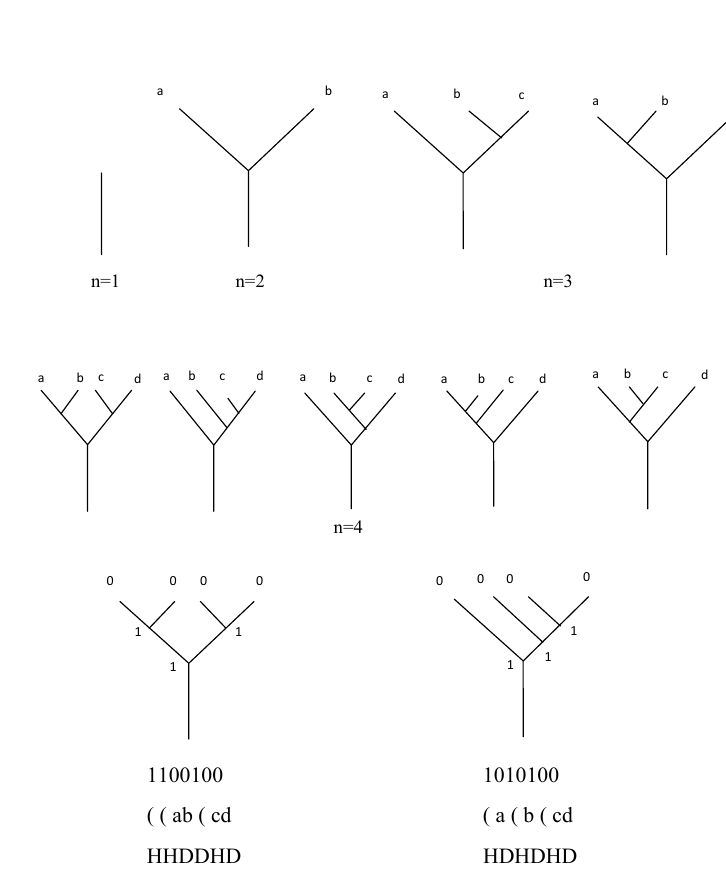
\includegraphics[width=1\linewidth]{../images/tri-trees}
\caption{Trivalent, planted trees with \(n\) leaves.\label{trivalenttrees}}
\end{figure}
\begin{figure}
\centering
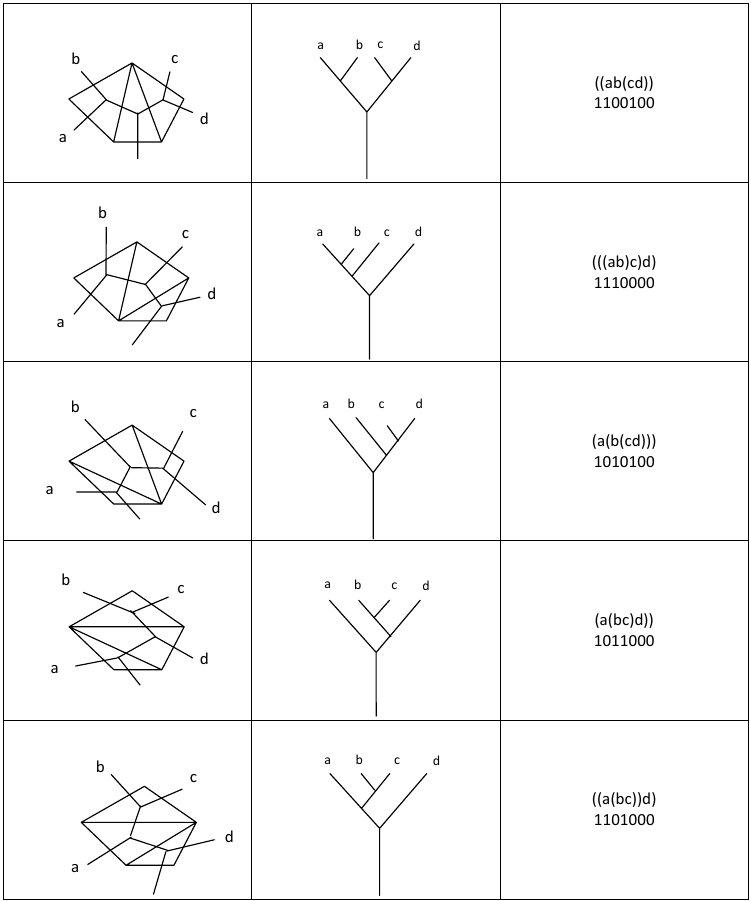
\includegraphics[width=1\linewidth]{../images/catalan-bijections.png}
\caption{\label{catalanbijections}}
\end{figure}
\typeout{************************************************}
\typeout{Exercises 2 Problems on Catalan Numbers}
\typeout{************************************************}
\section[{Problems on Catalan Numbers}]{Problems on Catalan Numbers}\label{exercises-2}
\begin{exerciselist}
\item[1.]\hypertarget{exercise-24}{}Use the recursion for \(P_{n}\) and compute \(P_{6}\), and \(P_{7}\).%
\par\smallskip
\item[2.]\hypertarget{exercise-25}{}Use the closed formula for \(P_n\) and compute \(P_{6}\) and \(P_{7}\).%
\par\smallskip
\item[3.]\hypertarget{exercise-26}{}Use \(G = P_{1}x + P_{2}x^{2} +\cdots\) and the recursion for \(P_{n}\) to determine a closed formula for \(P_{n}\).%
\par\smallskip
\item[4.]\hypertarget{prob-workseq}{}List the workable sequences for \(n = 4\).%
\par\smallskip
\item[5.]\hypertarget{prob-parenth}{}List the \(P_{6}\) ways of parenthesizing \(abcdef\).%
\par\smallskip
\item[6.]\hypertarget{exercise-29}{}Display a bijection between the 14 sequences in \hyperlink{prob-workseq}{Problem~4} and the 14 products in \hyperlink{prob-parenth}{Problem~5}.%
\par\smallskip
\item[7.]\hypertarget{exercise-30}{}Find the nonworkable sequence associated with each: \leavevmode%
\begin{enumerate}[label=(\alph*)]
\item\hypertarget{li-11}{}H H H D D H%
\item\hypertarget{li-12}{}D H H H H D%
\item\hypertarget{li-13}{}D D D H H H H H%
\item\hypertarget{li-14}{}D D H H D H H H%
\end{enumerate}
%
\par\smallskip
\item[8.]\hypertarget{exercise-31}{}Draw the \(T_{6}\) triangulations of a convex hexagon.%
\par\smallskip
\item[9.]\hypertarget{exercise-32}{}Display a bijection between the 5 ways of parenthesizing \(abcd\) and the 5 triangulations of a convex pentagon.%
\par\smallskip
\item[10.]\hypertarget{exercise-33}{}Let \(C_{n} = \frac{1}{n + 1}\binom{2n}{n}.\) Verifiy the formula:%
\begin{equation*}
C_{n} = \binom{n}{1} C_{n - 1} - \binom{n - 1}{2} C_{n - 2} + \binom{n - 2}{3} C_{n - 3} - \cdots
\end{equation*}
%
\par\smallskip
\item[11.]\hypertarget{exercise-34}{}Verify that \(H_{3} = 5\) by drawing the required paths.%
\par\smallskip
\item[12.]\hypertarget{exercise-35}{}Assign the appropriate binary sequences to each of the 5 trees for \(n=3\) in \hyperref[trivalenttrees]{Figure~\ref{trivalenttrees}}.%
\par\smallskip
\end{exerciselist}
\hypertarget{exercisegroup-1}{}\par\noindent For each of the following, investigate bijections that relate one to another.%
\begin{exercisegroup}(1)
\exercise[13.]\hypertarget{exercise-36}{}A and B each receive \(n\) votes. Let \(V_{n}\) denote the number of ways that the \(2n\) votes can be tallied so that A never trails B. Let \(V_{0} = 1\).%
\exercise[14.]\hypertarget{exercise-37}{}Place \(2n\) points on the circumference of a circle and draw \(n\)  nonintersecting chords in \(D_{n}\) ways; \(D_{0} = 1\)%
\exercise[15.]\hypertarget{exercise-38}{}In how many ways can \(1, 2, 3, \ldots, 2n\) be inserted into a \(2\times n\) rectangle such that the entries are increasing in rows and columns.  Let the answer be \(Y_n\); \(Y_1 = 1\), \(Y_2 = 2\).%
\exercise[16.]\hypertarget{exercise-39}{}Place \(2n\) points on a line segment and join them in pairs by nonintersecting arcs above the segment. In how many ways can this be done? Call the answer \(S_{n}\); \(S_{1}=1\), \(S_{2}=2\).%
\exercise[17.]\hypertarget{exercise-40}{}A rook on an \(n + 1\) by \(n + 1\) chessboard must move from the lower left corner to the upper right corner never going above the diagonal. How many paths are possible? Let \(K_{n}\) be the answer.%
\exercise[18.]\hypertarget{exercise-41}{}On an \(n + 1\) by \(n + 1\) chessboard a king starts on the first row and moves one square forward or back along a fixed column and ends on the starting square after \(2n\) moves. In how many ways, \(G_{n}\) , can this be done?%
\exercise[19.]\hypertarget{exercise-42}{}Count the number of planar rhyme schemes for a stanza consisting of \(n\) lines. Joanne Growney showed in her doctoral thesis that the Bell numbers, which count all rhyme schemes, have the Catalan numbers as a subsequence and that these enumerate precisely the planar rhyme schemes. For example, of the \(B_4 = 15\) rhyme schemes, \(C_4 = 14\) are planar. The nonplanar one is given by \(abab\).%
\end{exercisegroup}
\par\smallskip\noindent
%
\backmatter
%
%
%% A lineskip in table of contents as transition to appendices, backmatter
\addtocontents{toc}{\vspace{\normalbaselineskip}}
%
\cleardoublepage
\pagestyle{empty}
\vspace*{\stretch{1}}
\centerline{This book was authored in PreTeXt.%
}
\vspace*{\stretch{2}}
\end{document}